\chapter{Results and discussion}

\section{Characteristics of q\textsubscript{1} - q\textsubscript{2} stability diagrams for one electron}

%\subsection{Comparison of simulation and determinant stability criterion}

We will start by looking at the stability diagrams for different $\nicefrac{\Omega_2}{\Omega_1}$ ratios. Starting with \ref{fig:stabil-eta=3}.

\begin{figure}[H]
\begin{subfigure}{.5\textwidth}
  \centering
  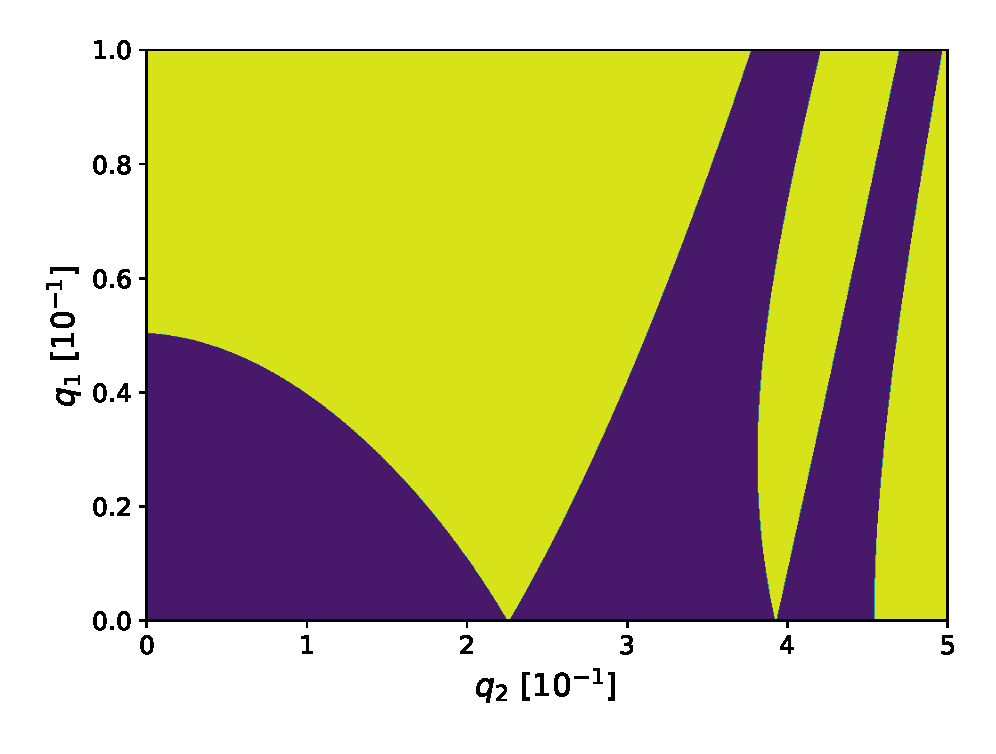
\includegraphics[width=\linewidth]{img/det_q1_0.0-0.1_q2_0.0-0.5_900x900_3.eps}
  \caption{Determinant}
  \label{fig:det_3}
\end{subfigure}%
\begin{subfigure}{.5\textwidth}
  \centering
  \includegraphics[width=\linewidth]{img/0_ions_1_electrons_q1_0.0-0.1_q2_0.0-0.5_960x960_3_100.eps}  
  \caption{Simulation}
  \label{fig:sim_3}
\end{subfigure}
\caption{Stability diagrams for $\nicefrac{\Omega_2}{\Omega_1} = 3$}
\label{fig:stabil-eta=3}
\end{figure}

In the sub-figure \ref{fig:det_3} we can see stable\textit{(dark)} and unstable\textit{(light)} regions of the studied differential equation. The image \ref{fig:sim_3} combines two pictures. The white curve indicates the edge of stability regions $\rightarrow$ the region under the curve is stable. In the background is a contour plot of the average electron velocity throughout the trajectory relative to the initial velocity. The color bar to the right indicates the value of this ratio. The figures such as \ref{fig:sim_3} can help us find the stable trap parameters while keeping electron temperature as low as possible, which is our ultimate goal. \xxx{In contrast with the determinant solution, we can see that the two stable areas for a simulated particle are cut off in the field with higher amplitudes. In the following figure, we increase the total simulation time and the diameter for identifying stable particles. And it doesn't work...}

Moving to larger frequency ratio $\rightarrow \nicefrac{\Omega_2}{\Omega_1} = 13$ we can start to notice some patterns.

\begin{figure}[H]
\begin{subfigure}{.5\textwidth}
  \centering
  \includegraphics[width=\linewidth]{img/det_q1_0.0-0.07_q2_0.0-0.5_960x960_13.eps}
  \caption{Determinant}
  \label{fig:det_13}
\end{subfigure}%
\begin{subfigure}{.5\textwidth}
  \centering
  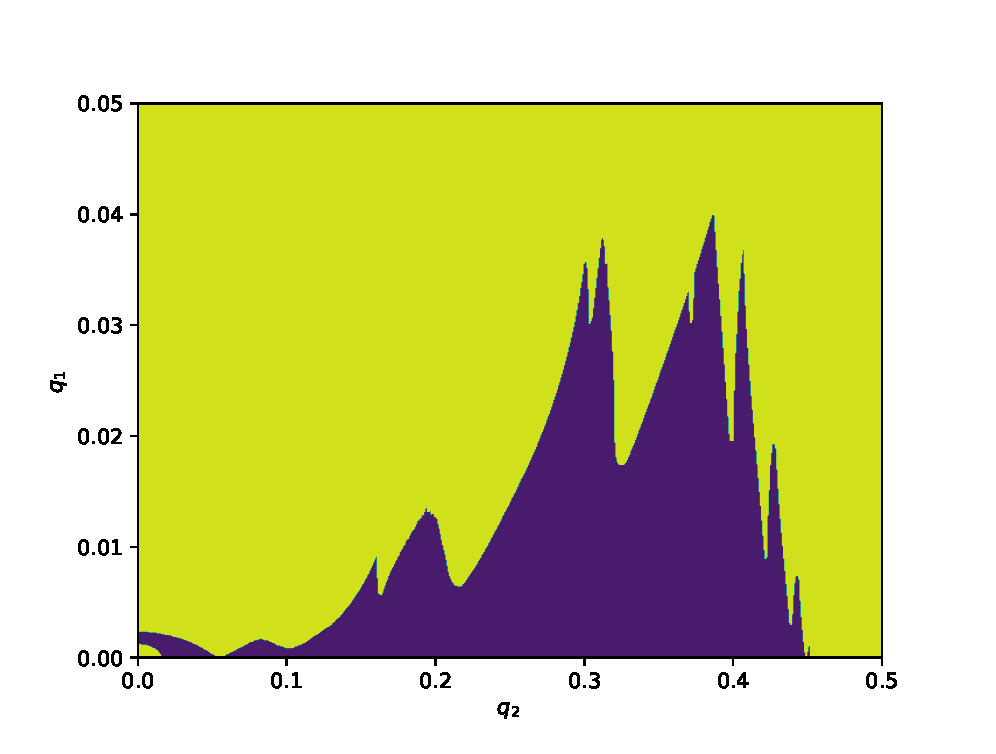
\includegraphics[width=\linewidth]{img/0_ions_1_electrons_q1_0.0-0.05_q2_0.0-0.5_640x640_13.eps}  
  \caption{Simulation}
  \label{fig:sim_13}
\end{subfigure}
\caption{Stability diagrams for $\nicefrac{\Omega_2}{\Omega_1} = 13$}
\label{fig:stabil-eta=13}
\end{figure}

There emerges one stable triangle with many tongues of instability. With an increasing ratio $\nicefrac{\Omega_2}{\Omega_1}$ we can see a gain in the number of these tongues, but their width promptly shrinks as well. We expect that by further increasing the frequency ratio, the unstable tongues will be realistically affecting only the regions near the edge of stability, leaving the regions further inside a stable triangle safe to work with.

\xxx{Continuing to the frequency ratio compatible for trapping electrons and Ca+ ions}

\begin{figure}[H]
	\centering
	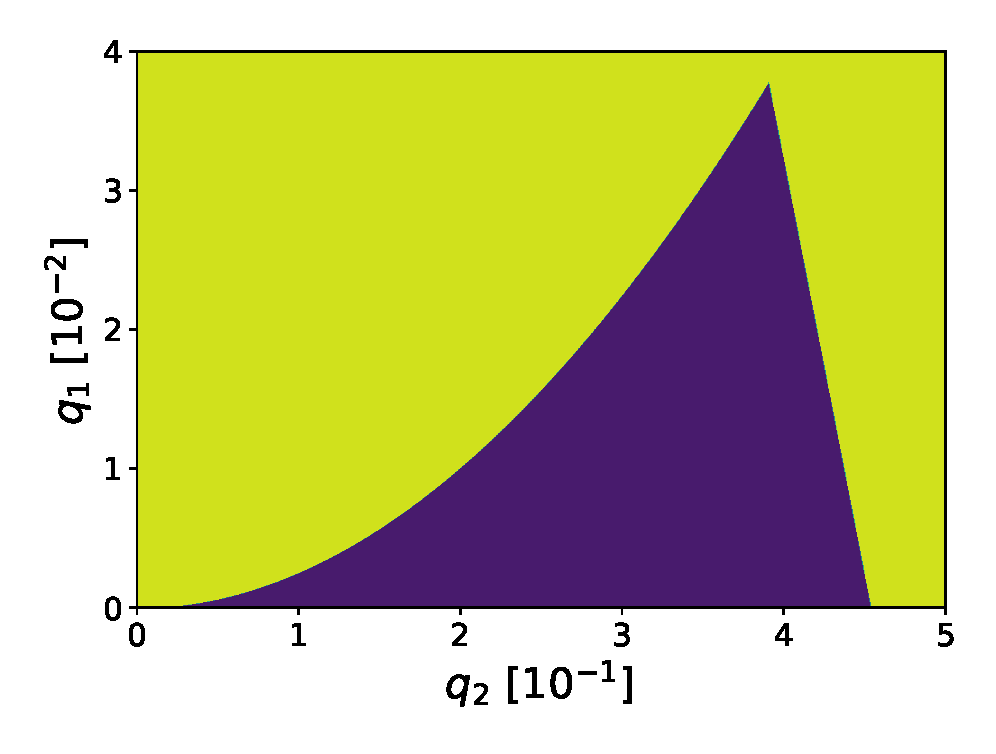
\includegraphics[width=\linewidth]{img/0_ions_1_electrons_q1_0.0-0.04_q2_0.0-0.5_897x897_833.eps}
	\caption{Simulated stability diagram for $\nicefrac{\Omega_2}{\Omega_1} = 833$}
	\label{fig:stabil-eta=833}
\end{figure}

\subsection{Dependence on initial conditions}

\begin{figure}[H]
\begin{subfigure}{.3\textwidth}
  \centering
  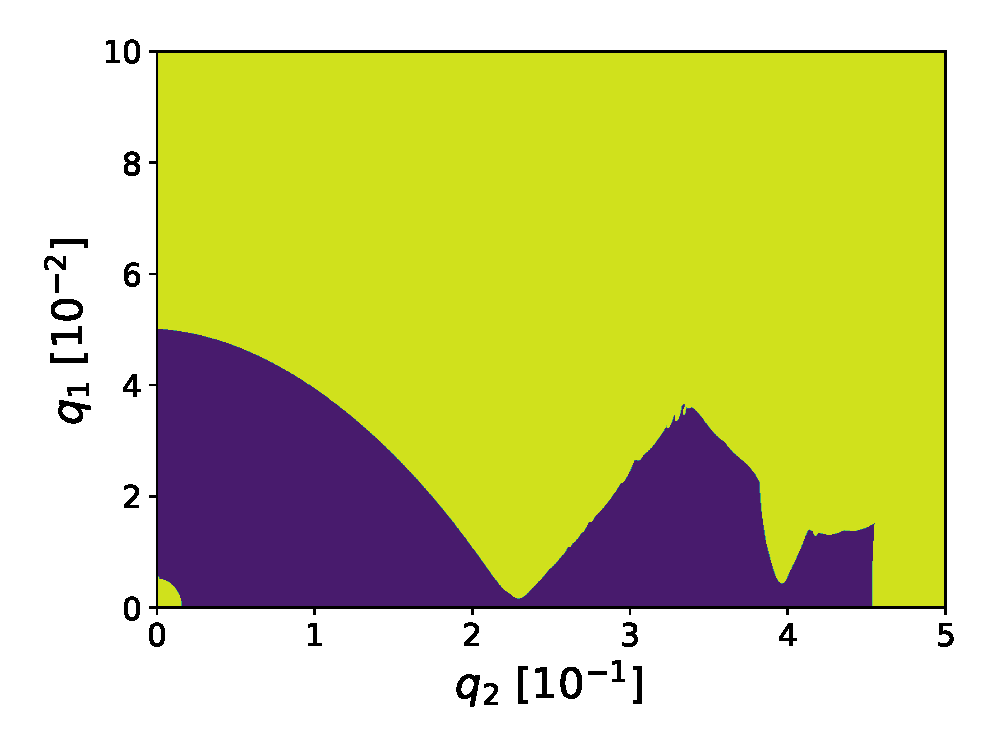
\includegraphics[width=\linewidth]{img/0_ions_1_electrons_q1_0.0-0.1_q2_0.0-0.5_960x960_3.eps}
  \caption{Normal initial conditions}
  \label{fig:normal_conds-3}
\end{subfigure}%
\begin{subfigure}{.3\textwidth}
  \centering
  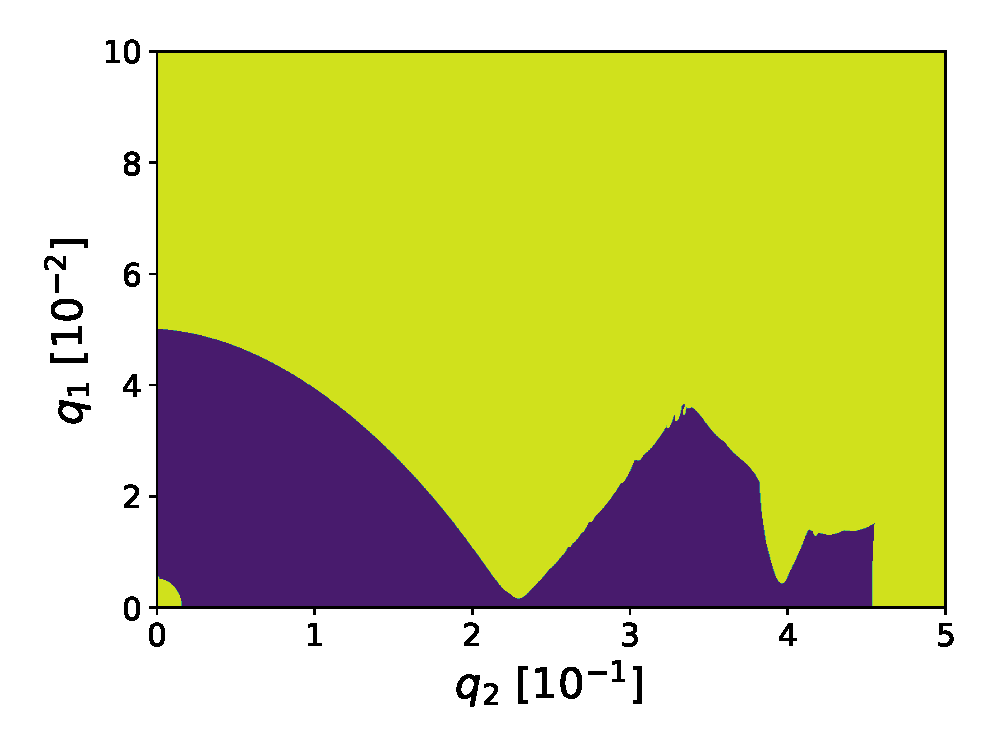
\includegraphics[width=\linewidth]{img/0_ions_1_electrons_q1_0.0-0.1_q2_0.0-0.5_960x960_3.eps}
  \caption{High velocity}
  \label{fig:high_velocity-3}
\end{subfigure}%
\begin{subfigure}{.3\textwidth}
  \centering
  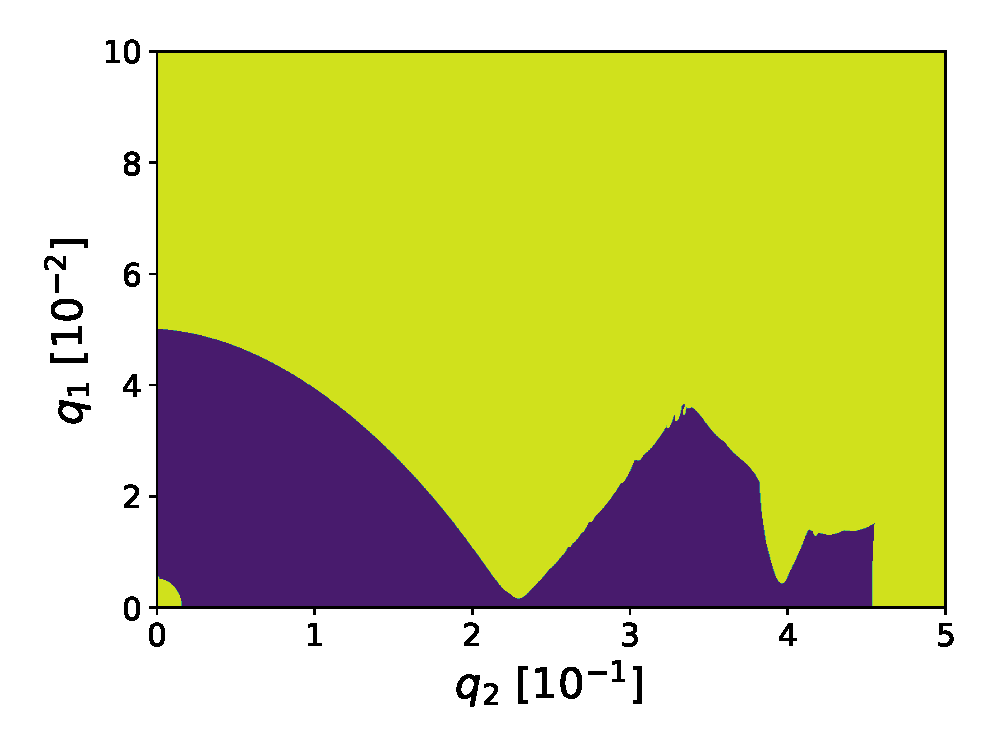
\includegraphics[width=\linewidth]{img/0_ions_1_electrons_q1_0.0-0.1_q2_0.0-0.5_960x960_3.eps}  
  \caption{Further away from center}
  \label{fig:large_radius-3}
\end{subfigure}
\caption{$\nicefrac{\Omega_2}{\Omega_1} = 3$, different initial conditions}
\label{fig:init-conds-eta=3}
\end{figure}

High initial velocity \ref{fig:high_velocity-3} makes the region with the weakest field (around $q_1 \approx q_2 \approx 0$) unstable, which is understandable since the stability condition \xxx{reference} is not satisfied. A wider distance from the trap's center combined with the initial velocity pointing away from the trap \ref{fig:large_radius-3} distorts the stability diagram's shape significantly. 

\xxx{as a sanity check we try to reproduce a result from \cite{leefer2017investigation}.} 

\section{Creating a Coulomb crystal}
\xxx{currently making some useable pictures}

\section{Stability of electron in Coulomb crystal}
\subsection{One electron - one ion}
\subsection{One electron - twenty ions}
\subsection{One electron - a hundred ions}

\section{Design of the experiment}

\section{Future}
\label{chap:future}

Our concerns in the future will be reproducing results of this thesis for the real planar geometry of the trap used in our experiment. The potential of such a trap can be formulated in integral form utilizing Bessel functions, which will make our simulations much more computationally expensive. We need to derive equation of motion and identify parameters analogous to $a$, $q_1$ and $q_2$ which we had for ideal quadrupole trap. After that we can use our exiting program to study stability of particles in dependence on such parameters exactly as we did in this thesis. 